\chapter{Grundlagen}\label{chap:grundlagen}

Dieses Kapitel stellt das theoretische Fundament der späteren praktischen Arbeit vor. Zunächst werden die
mathematischen und algorithmischen Grundlagen der Computertomographie erläutert, bevor die \gls{cuda}-Plattform als
technische Basis eingeführt wird.

\section{Die Computertomographie}

\subsection{Mathematische Grundlagen der Computertomographie}

In diesem Abschnitt werden die mathematischen Grundlagen der Computertomographie behandelt. Es werden zunächst die
mathematischen Eigenschaften der Vorwärtsprojektion und das sich daraus ergebende Fourier-Schichten-Theorem erläutert.
Anschließend wird die Aufnahme der Projektionen mit Parallelstrahlen erklärt und die Aufnahme mit Fächerstrahlen
abgeleitet. Zum Schluss wird das Prinzip der Fächerstrahlen auf den dreidimensionalen Raum ausgeweitet, also auf die
Aufnahme mit Kegelstrahlen.

\subsubsection{Projektionen}

Schießt man einen Röntgenstrahl durch ein festes Objekt, wie beispielsweise biologisches Gewebe oder ein Metall, so wird
dieser Strahl je nach Dichte des Materials entlang seiner Bahn abgeschwächt bzw.\ absorbiert. Mathematisch lässt sich
ein Objekt als zwei- oder dreidimensionale Verteilung von Absorptionskonstanten verstehen, während die gesamte
Abschwächung entlang einer Strahlbahn als Kurvenintegral dargestellt werden kann.

Die Grundlage der folgenden Ausführungen ist die Abbildung~\ref{fig:math_proj}~\cite{kak}. Als Beispiel dienen ein
Objekt, dargestellt als die Funktion $f(x, y)$, sowie Kurvenintegrale, dargestellt durch das Parameterpaar
$(\alpha, t)$. Die Linie $AB$ lässt sich dann durch die folgende Formel darstellen:

\begin{equation*}
    x \cdot \cos \alpha + y \cdot \sin \alpha  = t_1
\end{equation*}

oder allgemein für beliebige, zu $AB$ parallele, Linien:

\begin{equation}\label{eq:proj_obj}
    x \cdot \cos \alpha + y \cdot \sin \alpha = t
\end{equation}

\begin{figure}[!htb]
\centering
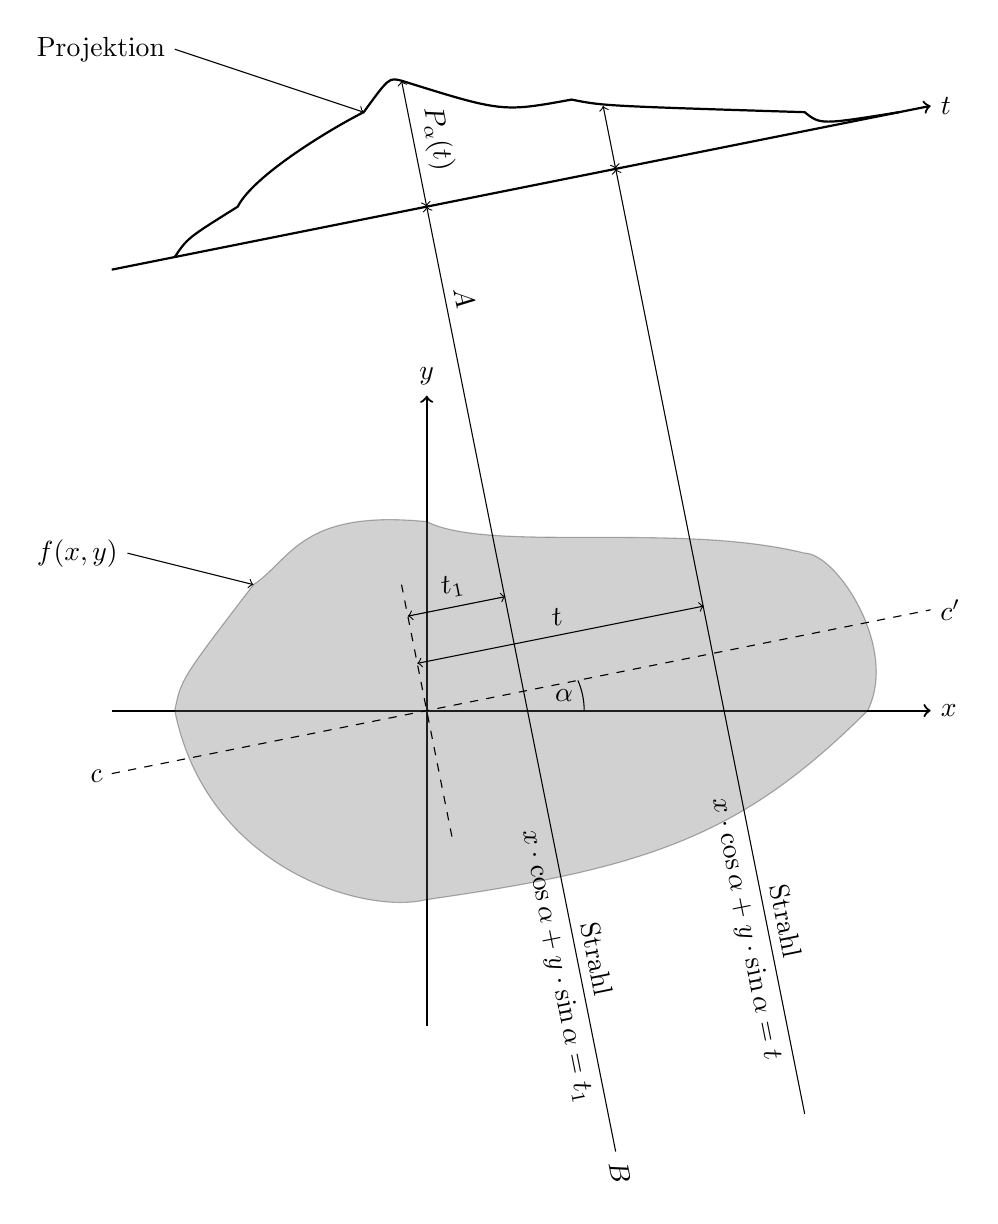
\begin{tikzpicture}[
    scale=0.8,
    axis/.style={thick,->}]
    % Achsen
    \draw[axis] (-5, 0) -- (8, 0) node[right] {$x$};
    \draw[axis] (0, -5) -- (0, 5) node[above] {$y$};
    \draw[axis] (-5, 7) -- (8, 9.6) node[right,sloped] {$t$};

    % Objekt
    \draw[fill=black!60!white,opacity=0.3] (0, -3) .. controls (3.5, -2.5) and (5, -2) .. (7, 0)
                                            .. controls (7.5, 1) and (6.5, 2.5) .. (6, 2.5)
                                            .. controls (4, 3) and (1, 2.5) .. (0,3)
                                            .. controls (-2, 3.2) and (-2.15, 2.4) .. (-2.75, 2)
                                            .. controls (-3.9, 0.5) .. (-4, 0)
                                            .. controls (-3.5, -2.5)  and (-1, -3.25) .. (0, -3);

    % Strahlen
    \draw[->] (3, -7) -- (0, 8) node[pos=0.9,above,sloped] {$A$} node[pos=0.2,above,sloped] {Strahl}
              node[pos=0.2,below,sloped] {$x \cdot \cos \alpha + y \cdot \sin \alpha = t_1$} node[pos=0,right,sloped] {$B$};

    \draw[->] (6, -6.4) -- (3, 8.6) node[pos=0.2,above,sloped] {Strahl}
              node[pos=0.2,below,sloped] {$x \cdot \cos \alpha + y \cdot \sin \alpha = t$};

    % t
    \draw[<->] (-0.3, 1.5) -- (1.25, 1.81) node[pos=0.5,above,sloped] {$t_1$};
    \draw[<->] (-0.15, 0.75) -- (4.4, 1.66) node[pos=0.5,above,sloped] {$t$};

    % sonstiges
    \draw[dashed] (-5, -1) -- (8, 1.6) node[pos=0,sloped,left] {$c$} node[sloped,right] {$c'$};
    \draw[dashed] (0.4, -2) -- (-0.4, 2);

    % Projektion
    \draw[<->] (0, 8) -- (-0.4, 10) node[pos=0.5, sloped, above] {$P_{\alpha}(t)$};
    \draw[<->] (3, 8.6) -- (2.8, 9.6);
    \draw[thick] (-4, 7.2) .. controls (-3.8, 7.5) .. (-3, 8)
                 .. controls (-2.75, 8.5) and (-1.5, 9.25) .. (-1, 9.5)
                 .. controls (-0.6, 10.05) .. (-0.4, 10)
                 .. controls (1.2, 9.5) .. (2.3, 9.7)
                 .. controls (2.8, 9.6) .. (6, 9.5)
                 .. controls (6.25, 9.3) .. (7.5, 9.5);

    % Beschriftungen
    \draw[->] (-4.75, 2.5) -- (-2.75, 2) node[pos=0,left] {$f(x, y)$};
    \draw[->] (-4, 10.5) -- (-1, 9.5) node[pos=0, left] {Projektion};

    % Winkel
    \draw (2.5, 0) arc (0:23.5:12mm) node[pos=0.5,left] {$\alpha$};
\end{tikzpicture}
\caption{Zusammenhang zwischen Linienintegral und Projektion}
\label{fig:math_proj}
\end{figure}

Das zu $f(x, y)$ gehörige Linienintegral ist $P_{\alpha}(t)$:

\begin{equation}\label{eq:proj_int}
    P_{\alpha}(t) = \int\limits_{(\alpha, t)} f(x, y) \mathrm{d}s
\end{equation}

Zusammen mit der aus Formel~\ref{eq:proj_obj} resultierenden Delta-Distribution lässt sich das Linienintegral wie folgt
umschreiben:

\begin{equation}\label{eq:proj_radon}
    P_{\alpha}(t) = \int\limits_{-\infty}^{\infty}\int\limits_{-\infty}^{\infty}f(x, y) \cdot \delta(x \cdot
                    \cos \alpha + y \cdot \sin \alpha - t) \mathrm{d}x \mathrm{d}y
\end{equation}

Die Funktion $P_{\alpha}(t)$ ist die \textit{Radon-Transformation} der Funktion $f(x, y)$~\cite{radon}.

Eine Projektion lässt sich als die Kombination einer Menge von Radon-Transformationen verstehen. Die
(mathematisch) einfachste Projektion ist eine Sammlung von Parallelstrahlintegralen $P_{\alpha}(t)$ unter einem
konstanten Winkel $\alpha$. Man bezeichnet eine solche Projektion als \textit{Parallelstrahlprojektion} (siehe
Abbildung~\ref{fig:par_proj}). In der Praxis kann eine Parallelstrahlprojektion durch die Bewegung einer
Quelle-Detektor-Anordnung entlang paralleler Linien auf entgegengesetzten Seiten des Objekts aufgenommen werden.

Eine zweite Aufnahmemöglichkeit ist der Einsatz einer Quelle auf einer festen Position sowie einer Reihe von Detektoren
entlang einer Linie auf der anderen Seite des Objekts (siehe Abbildung~\ref{fig:fan_proj}). Solcherart erzeugte
Projektionen nennt man aufgrund der fächerförmigen Strahlen \textit{Fächerstrahlprojektionen}~\cite{kakslan}.

\subsubsection{Das Fourier-Schichten-Theorem}

Betrachtet man die eindimensionale 

\subsubsection{Parallelstrahlen}

\subsubsection{Fächerstrahlen}

\subsubsection{Kegelstrahlen}

\subsection{Die prinzipielle Funktionsweise der Computertomographie}

Am Anfang der Computertomographie steht das Röntgenverfahren, das 1895 vom deutschen Physiker Wilhelm Conrad Röntgen
entdeckt wurde~\cite{roentgen}. Mit Hilfe einer Strahlungsquelle wird ein Objekt durchleuchtet und auf einem Film bzw.\
einem Detektor abgebildet; der dreidimensionale Körper wird also auf eine zweidimensionale Fläche projiziert. Diesen
Schritt bezeichnet man als \textit{Vorwärtsprojektion}.

Führt man die Vorwärtsprojektion genügend oft in aufeinanderfolgenden Winkelschritten aus, bis man (idealerweise) einen
Vollkreis abgefahren hat, so lässt sich aus den dabei entstandenen \textit{Projektionen} der ursprünglich durchleuchtete
Körper, den wir in der Folge als \textit{Volumen} bezeichnen, rekonstruieren. Für jeden Punkt im Volumen
(\textit{\gls{voxel}}) kann anhand der Informationen aus den Projektionen der Absorptionsgrad berechnet und dadurch die
innere Struktur des Volumens bestimmt werden. Dieser Zusammenhang wurde in den 60er Jahren des 20. Jahrhunderts durch
den südafrikanisch-amerikanischen Physiker Allan McLeod Cormack festgestellt, der ebenfalls die dazu notwendigen
mathematischen Grundlagen entwickelte~\cite{cormack63}~\cite{cormack64}; ihm war allerdings unbekannt~\cite{cormack79},
dass diese schon 1917 vom österreichischen Mathematiker Johann Radon gefunden wurden~\cite{radon}. Mathematisch ist der
Vorgang der \textit{Rückprojektion} eine Anwendung der nach Radon benannten \textit{Radon-Transformation}.

Ein Problem der Vorwärtsprojektion ist der Informationsverlust, der durch die mangelnde Tiefe des Films bzw.\ Detektors
entsteht; die Tiefeninformationen werden auf die zweidimensionale Fläche {\glqq}verschmiert{\grqq}. Bei der
Rückprojektion lässt sich dieser Verlust durch die Wahl eines geeigneten Bildfilters wiederum kaschieren, weshalb man
auch von der \textit{gefilterten Rückprojektion} spricht.

Da die gefilterte Rückprojektion für jedes \gls{voxel} einzeln berechnet werden muss, ist sie für einen Menschen nicht
in sinnvoller Zeit lösbar. Aus diesem Grund ist man für die Lösung des Gesamtproblems auf einen Computer angewiesen,
woraus sich der Name des Verfahrens ableitet: \textit{Computertomographie}. Die ersten bis zur Marktreife entwickelten
Computertomographen wurden gegen Ende der 60er Jahre des 20. Jahrhunderts vom englischen Elektroingenieur Godfrey
Hounsfield gebaut. Dieser entwickelte die für die Rückprojektion nötigen Algorithmen ebenfalls selbst, da ihm die
Vorarbeiten von Cormack und Radon nicht bekannt waren~\cite{kalender}. Für ihre voneinander unabhängigen Arbeiten
erhielten Godfrey und Cormack 1979 den Nobelpreis für Physiologie oder Medizin, was die Bedeutung der
Computertomographie insbesondere für die Medizin unterstreicht.

\subsection{Der Feldkamp-Davis-Kress-Algorithmus}

Der 1984 entwickelte \gls{fdk}~\cite{fdk} ist eine spezielle Ausprägung der gefilterten Rückprojektion für die
Computertomographie mit Kegelstrahlen. In diesem Abschnitt wird zunächst die zugrundeliegende Geometrie näher erläutert,
bevor die einzelnen Schritte des \gls{fdk} detaillierter betrachtet werden.

\subsubsection{Geometrie}\label{sssec:fdk_geometrie}

 Der Ausgangspunkt der Strahlung ist eine Quelle $S$ (\textit{source}), die das
Volumen $O$ (\textit{object}) unter einem Drehwinkel $\alpha_p$ mit einem \textit{kegelförmigen} Strahl durchleuchtet
und auf einem Detektor mit $N_h \cdot N_v$ \gls{pixel}n abbildet. Dabei stellt $d_{src}$ den Abstand zwischen der Quelle
und dem Rotationsmittelpunkt, also dem Zentrum des durchleuchteten Volumens, dar, während $d_{det}$ den Abstand zwischen
dem Rotationsmittelpunkt und dem Detektor bezeichnet (vgl. Abbildung~\ref{fig:fdk_geometrie}).

\begin{figure}[!htb]
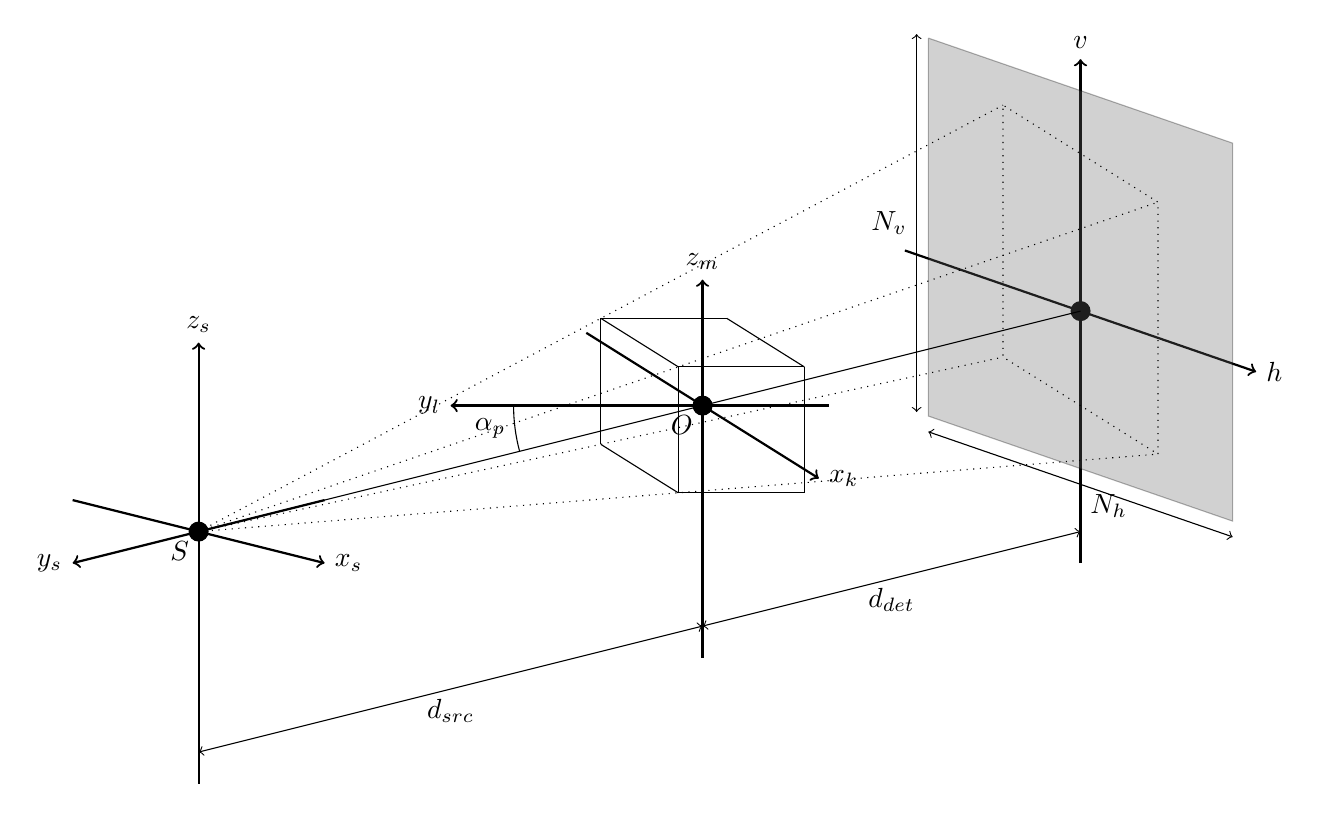
\begin{tikzpicture}[
        scale=0.8,
        axis/.style={thick,->}
    ]
    % Quelle
    \coordinate (1) at (0, 0, 0);
    \filldraw[fill=black,draw=black] (1) circle (0.15cm) node[below left] {$S$};
    \draw[axis] (-2, 0.5, 0) -- (2, -0.5, 0) node[right] {$x_s$};
    \draw[axis] (2, 0.5, 0) -- (-2, -0.5, 0) node[left] {$y_s$};
    \draw[axis] (0, -4, 0) -- (0, 3, 0) node[above] {$z_s$};

    % Volumen
    \coordinate (2) at (8, 2, 0);
    \filldraw[fill=black,draw=black] (2) circle (0.15cm) node[below left] {$O$};
    \draw[axis] (5, 2, -3) -- (11, 2, 3) node[right] {$x_k$};
    \draw[axis] (10, 2, 0) -- (4, 2, 0) node[left] {$y_l$};
    \draw[axis] (8, -2, 0) -- (8, 4, 0) node[above] {$z_m$};

    \draw (8, 1, 1) -- (10, 1, 1);
    \draw (8, 1, 1) -- (8, 3, 1);
    \draw (8, 1, 1) -- (6, 1, -1);

    \draw (8, 3, 1) -- (10, 3, 1);
    \draw (8, 3, 1) -- (6, 3, -1);

    \draw (10, 1, 1) -- (10, 3, 1);

    \draw (6, 1, -1) -- (6, 3, -1);

    \draw (6, 3, -1) -- (8, 3, -1);

    \draw (10, 3, 1) -- (8, 3, -1);


    % Detektor
    \coordinate(3) at (14, 3.5, 0);
    \filldraw[fill=black,draw=black] (3) circle (0.15cm);
    \draw[axis] (10.25, 3.5, -2.5) -- (17.75, 3.5, 2.5) node[right] {$h$};
    \draw[axis] (14, -0.5, 0) -- (14, 7.5, 0) node[above] {$v$};
    \draw[fill=black!60!white,opacity=0.3] (10.75, 7, -2.16666) -- (17.25, 7, 2.16666) -- (17.25, 1, 2.16666)
                                           -- (10.75, 1, -2.16666) -- (10.75, 7, -2.16666);
    \draw[<->] (10.5, 1, -2.33333) -- (10.5, 7, -2.33333) node[pos=0.5, left] {$N_v$};
    \draw[<->] (10.75, 0.75, -2.16666) -- (17.25, 0.75, 2.16666) node[pos=0.5, below right] {$N_h$};

    % Abstände
    \draw (1) -- (3);
    \draw[<->] (0, -3.5, 0) -- (8, -1.5, 0) node[pos=0.5,below] {$d_{src}$};
    \draw[<->] (8, -1.5, 0) -- (14, 0, 0) node[pos=0.5,below] {$d_{det}$};

    % Kegelstrahlen
    \draw[dotted] (1) -- (16, 2, 2);
    \draw[dotted] (1) -- (16, 6, 2);
    \draw[dotted] (1) -- (12, 2, -2);
    \draw[dotted] (1) -- (12, 6, -2);

    % Kegelstrahlenabbild
    \draw[dotted] (16, 2, 2) -- (16, 6, 2) -- (12, 6, -2) -- (12, 2, -2) -- (16, 2, 2);

    % Winkel
    \draw (5, 2, 0) arc (180:195:2.8cm) node[pos=0.5, left] {$\alpha_p$};
\end{tikzpicture}
\caption{Geometrie der gefilterten Rückprojektion}
\label{fig:fdk_geometrie}
\end{figure}

\subsubsection{Wichtung}\label{sssec:fdk_wichtung}

Nach der Aufnahme wird jede Projektion gewichtet. Dafür wird jedes \gls{pixel} mit den Koordinaten $(j, i)$ mit dem
Wichtungsfaktor $w_{ij}$ multipliziert.

\begin{equation}\label{eq:wichtung}
    w_{ij} = \frac{d_{det} - d_{src}}{\sqrt{(d_{det} - d_{src})^2 + h_j^2 + v_i^2}}
\end{equation}

\subsubsection{Filterung}\label{sssec:fdk_filter}

Zum Ausgleich der durch die Vorwärtsprojektion verloren gegangenen Tiefeninformationen werden die Projektionen im
nächsten Schritt zeilenweise gefiltert. Zu diesem Zweck müssen die Projektionen und der Filter allerdings mittels der
diskreten Fouriertransformation in den komplexen Raum transformiert werden; zum Einsatz kommt dabei das Verfahren der
schnellen Fouriertransformation (\textit{fast Fourier transform}, FFT) nach Cooley und Tukey~\cite{cooltuk}. Da dieses
Verfahren nur mit einer Menge von Elementen funktioniert, die einer Zweierpotenz entspricht, müssen die
Projektionszeilen und der Filter auf die nächste Zweierpotenz {\glqq}aufgerundet{\grqq} werden. Dazu wird, ausgehend von
der Länge einer Projektionszeile $N_h$,  die Filterlänge $N_{hFFT}$ berechnet:

\begin{equation}
    N_{hFFT} = 2 \cdot 2^{\left\lceil \log_{2} N_h \right\rceil}
\end{equation}

Mit der so bestimmten Filterlänge lässt sich der Filter $r$ erzeugen:

\begin{equation}\label{eq:filter_gen}
    \begin{aligned}
        r(j) \text{ mit } j &\in \left[-\frac{N_{hFFT} - 2}{2}, \frac{N_{hFFT}}{2}\right]\\
        r(j) &=
            \begin{cases}
                \frac{1}{8} \cdot \frac{1}{\tau^2} & \quad \text{wenn } j = 0\\
                0 & \quad \text{wenn } j \text{ gerade}\\
                -\frac{1}{2j^2\pi^2\tau^2} & \quad \text{wenn } j \text{ ungerade}\\
            \end{cases}
    \end{aligned}
\end{equation}

Nun wird die zu filternde Zeile so lange mit $0$ aufgefüllt, bis die erweiterte Zeile $N_{hFFT}$ \gls{pixel} umfasst:

\begin{equation}
    \begin{aligned}
        p &: \text{ mit Nullen aufgefüllte Projektionszeile}\\
        p(0 \dots N_{h - 1}) &= \text{det}(0 \dots N_{h - 1})\\
        p(N_{h} \dots N_{hFFT}) &= 0
    \end{aligned}
\end{equation}

Im Anschluss werden sowohl der Filter $r$ als auch die erweiterte Projektionszeile $p$ in den komplexen Raum
transformiert und dort miteinander multipliziert:

\begin{equation}
    \begin{aligned}
        R &= \text{FFT}(r)\\
        P &= \text{FFT}(p)\\
        F &= P \cdot R \quad \text{sowohl für den reellen als auch den imaginären Teil}
    \end{aligned}
\end{equation}

Die so gefilterte Projektionszeile $F$ wird dann mit der inversen schnellen Fouriertransformation (IFFT) in den
reellen Raum zurücktransformiert und von den {\glqq}aufgefüllten{\grqq} Elementen bereinigt:

\begin{equation}
    \begin{aligned}
        f &= \text{IFFT}(F)\\
        \text{gefilterte Projektionszeile} &: f(0 \dots N_{h - 1})
    \end{aligned}
\end{equation}

\subsubsection{Rückprojektion}

Die auf gefilterten Projektionen können nun nach dem folgenden Algorithmus für die Rückprojektion verwendet werden:

Für jede Projektion $p$ mit dem Drehwinkel $\alpha_p$:

\begin{itemize}
    \item berechne für jede \gls{voxel}koordinate $(x_k, y_l, z_m)$ deren rotierte Position $(s, t, z)$:
        \begin{equation}
            \begin{aligned}
                s &= x_k \cos \alpha_p + y_l \sin \alpha_p\\
                t &= -x_k \sin \alpha_p + y_l \cos \alpha_p\\
                z &= z_m
            \end{aligned}
        \end{equation}

    \item projiziere die rotierte \gls{voxel}koordinate $(s, t, z)$ auf den Detektor:
        \begin{equation}
            \begin{aligned}
                h' &= y' = t \cdot \frac{d_{det} - d_{src}}{s - d_{src}}\\
                v' &= z' = z \cdot \frac{d_{det} - d_{src}}{s - d_{src}}
            \end{aligned}
        \end{equation}

    \item interpoliere das Detektorsignal bei $(h', v')$:
        \begin{equation}
            \begin{aligned}
                det' = det(h', v')
            \end{aligned}
        \end{equation}

    \item führe die Rückprojektion für jedes \gls{voxel} $vol_{klm}$ aus:
        \begin{equation}
            \begin{aligned}
                vol_{klm} &= vol_{klm} + 0,5 \cdot det' \cdot u^2\\
                \text{mit } u &= \frac{d_{src}}{s - d_{src}}
            \end{aligned}
        \end{equation}
\end{itemize}

Nach Abschluss der Rückprojektion erhält man ein Volumen, dessen \gls{voxel} Aufschluss über seine innere Struktur
geben.

\subsection{Bisherige Parallelisierungsansätze}\label{ssec:par}

Aufgrund seiner geringen Komplexität und einfachen Implementierbarkeit ist der \gls{fdk} einer der beliebtesten
Rückprojektionsalgorithmen für die Kegelstrahl-Computertomographie~\cite{xumuell}. Der Vorteil des \gls{fdk} liegt
außerdem darin, dass die gefilterte Rückprojektion für jedes \gls{voxel} individuell berechnet werden kann, das heißt
ohne Abhängigkeiten zu anderen \gls{voxel}n. Dieser Umstand ermöglicht für die maschinelle Berechnung den maximalen Grad
an Parallelität, der im englischen Sprachraum auch als \textit{embarassingly parallel} bezeichnet wird, und macht den
\gls{fdk} zu einem idealen Ziel für diverse Parallelisierungsansätze. Einige neuere Ansätze sollen im Folgenden
vorgestellt werden.

Seit seiner Einführung ist der \gls{fdk} ein beliebtes Untersuchungsobjekt diverser Forschungsgruppen, die sich mit
seiner Beschleunigung bzw.\ Parallelisierung mittels einer großen Variation von Architekturen, Plattformen und
Programmiermodellen beschäftigen. 

Xu et al.\ untersuchten bereits 2004, inwieweit sich der \gls{fdk} durch den Einsatz handelsüblicher Grafikkarten
(\textit{commodity graphics hardware}) beschleunigen lässt~\cite{xumuell}. Dabei wurden die Schritte \textit{Wichtung}
und \textit{Filterung} aufgrund ihrer geringen Komplexität ($\mathcal{O}(n^2)$) auf der \gls{cpu} ausgeführt, während
man die komplexere \textit{Rückprojektion} ($\mathcal{O}(n^4)$) auf der \gls{gpu} berechnete. Die Rückprojektion fand
schichtweise statt, jeweils für eine \gls{voxel}ebene entlang der vertikalen Volumenachse. In ihrem Fazit stellten die
Autoren die Vermutung auf, dass der Abstand zwischen den Leistungen von \gls{cpu}s und \gls{gpu}s in der Zukunft
zugunsten der \gls{gpu}s immer größer werden würde: \textit{Since GPU performance has so far doubled every 6 months 
(i.e., triple of Moore's law), we expect that the gap between CPU and GPU approaches will widen even further in the near
future.}

Li et al.\ beschäftigten sich 2005 damit, wie man den \gls{fdk} mit einem \gls{fpga} implementieren könnte. Dazu teilten
sie das Ausgabevolumen, also die Zieldaten der Rückprojektion, in mehrere Würfel (\textit{bricks}) auf, um zu einer
optimalen Cachenutzung zu kommen. Der verwendete deterministische Aufteilungsalgorithmus hatte zur Folge, dass bei der
Berechnung auf dem \gls{fpga} kein Cache-Verfehlen (\textit{cache miss}) mehr auftrat.

Knaup et al.\ gingen 2007 der Frage nach, ob der \gls{fdk} durch die Eigenschaften der Cell-Architektur profitieren
könne~\cite{knaupsteck}.

Scherl et al.\ unternahmen 2008 den Versuch, den \gls{fdk} mittels \gls{cuda} zu beschleunigen~\cite{scherlkeck}. Im
Gegensatz zu der Gruppe um Xu et al.\ führten sie alle Schritte auf der \gls{gpu} aus und führten die Rückprojektion
projektionsweise durch, das heißt, dass jede Projektion einzeln in das Gesamtvolumen zurückprojiziert wurde. Diese Art
der Datenverarbeitung ermöglichte es, die Schritte \textit{Wichtung} und \textit{Filterung} parallel zur Rückprojektion
auszuführen. Zur Ausnutzung dieser Eigenschaft und zur besseren Kapselung bzw.\ Modularisierung der Teilschritte
entwickelten die Autoren daher eine Pipeline-Struktur zur parallelen Abarbeitung des Algorithmus, basierend auf dem von
Mattson et al.\ vorgestellten Entwurfsmuster~\cite{mattsan}.

Balász et al.\ versuchten 2009 das Gleiche mit der \gls{opencl}~\cite{balgab}.

Hofmann et al.\ untersuchten eventuelle Vorteile durch den Einsatz der neuen Koprozessoren vom Typ 
Intel{\textregistered} Xeon Phi{\texttrademark} {\glq}Knights Corner{\grq}~\cite{hoftrei}.

Zhao et al.\ verfolgten die Absicht, eine Beschleunigung durch Ausnutzung geometrischer Zusammenhänge zu
erreichen~\cite{zhao}. Sie setzten dabei auf die Tatsache, dass ein einmal bestimmtes, also auf den Detektor
projiziertes, \gls{voxel} durch Rotation in 90°-Schritten die rotierten \gls{voxel} ebenfalls genau bestimmt. Ist also
für ein \gls{voxel} im Projektionswinkel 0° die zugehörige Detektorkoordinate gefunden, so kann diese Detektorkoordinate
für die Projektionswinkel 90°, 180° und 270° und die entsprechenden \gls{voxel} wiederverwendet werden.

\section{Die NVIDIA{\textregistered}-CUDA{\textregistered}-Plattform}

\subsection{Programmierbare Grafikkarten}\label{ssec:cu_prog_gpu}

Als NVIDIA{\textregistered} im Jahre 2006 seine \textit{Compute-Unified-Device-Architecture}-Plattform
(CUDA{\textregistered}) vorstellte, die die direkte Programmierung der NVIDIA{\textregistered}-Grafikkarten ermöglichte,
folgte die Firma damit einer Entwicklung, die in den ersten Jahren des neuen Jahrtausends begonnen hatte. Durch die
Einführung von dezidierten Berechnungseinheiten für Gleitkommazahlen (\gls{fpu}) sowie den zunehmenden Funktionsumfang
der auf den Grafikkarten verbauten Shader-Einheiten wurde es theoretisch möglich, Berechnungen, die vorher nur von
\gls{cpu}s ausgeführt werden konnten, nun auch von \gls{gpu}s ausführen zu lassen. Dabei haben Grafikkarten gegenüber
herkömmlichen Prozessoren den Vorteil, dass die auf ihnen ausgeführten Berechnungen aufgrund ihrer für die
Computergrafik optimierten Bauweise -- also die Manipulation vieler \gls{pixel} zur gleichen Zeit -- automatisch
\textit{datenparallel} sind. \textit{Datenparallelität} bezeichnet dabei die parallele Ausführung derselben Berechnung
bzw.\ Anweisung auf verschiedenen Daten. Dem gegenüber steht die \textit{Taskparallelität}, mit der eine parallele
Abarbeitung verschiedener Aufgaben gemeint ist. \textit{Taskparallelität} entspricht eher dem Programmiermodell der
klassischen \gls{cpu}, ist auf \gls{gpu}s aufgrund der ihnen inhärenten datenparallelen Funktionsweise nur begrenzt
anwendbar.

Die \textit{datenparallele} Berechnung auf \gls{gpu}s, meistens \gls{gpgpu} genannt, bietet sich insbesondere
für die Verarbeitung großer Datenmengen an, wie sie zum Beispiel in der Wissenschaft häufig vorkommt. Am Anfang der
2000er Jahre gab es allerdings keine komfortable Möglichkeit, die erhältlichen Grafikkarten direkt zu programmieren;
man war daher gezwungen, die zu berechnenden Daten zunächst in Objekte der Computergrafik umzuwandeln (beispielsweise 
Texturen) und mit den Mitteln der bestehenden Computergrafik-Bibliotheken wie der \gls{opengl} oder \gls{directx} zu
bearbeiten. Mit der Einführung von \gls{cuda} entfiel diese Beschränkung, da es nun möglich war, speziell für die
Grafikkarte geschriebene Programme auf dieser auszuführen, ohne den Umweg über Computergrafik-Bibliotheken gehen zu
müssen.

\subsection{Das \gls{cuda}-Programmier- und Ausführungsmodell}

\subsubsection{\gls{kernel} und \gls{device}-Funktionen}

Das Herzstück eines \gls{cuda}-Programms ist der \gls{kernel}, also ein speziell für die \gls{gpu} geschriebenes
Programmstück. Ein \gls{kernel} wird in einem C- oder C++-Dialekt geschrieben und durch den \gls{cuda}-eigenen Compiler
in den Maschinencode der jeweiligen Zielarchitektur übersetzt. Dieser \gls{kernel} kann dann, ähnlich einer normalen
Funktion, aus einem in C oder C++ geschriebenen Programm (dem \gls{host}) aufgerufen werden. Der so gestartete
\gls{kernel} wird dann durch die \gls{cuda}-Laufzeitumgebung auf der \gls{gpu} (dem \gls{device}) ausgeführt. Da der
\gls{kernel} nicht auf der CPU ausgeführt wird, ist sein Aufruf in Bezug auf den \gls{host} asynchron, das Ende der
Berechnung wird auf der \gls{host}seite also nicht abgewartet und erfordert eine manuelle Synchronisierung durch den
\gls{host}:

\begin{minted}[breaklines,breakafter=\,,fontsize=\small]{c++}
    auto main(int argc, char** argv) -> int
    {
        kernel<<<...,...>>>(...);
        // Host-Programm wird nach Kernelaufruf weiter ausgeführt
        // Kernel-Ergebnis kann noch nicht verwendet werden
        cudaDeviceSynchronize();
        // Kernel-Ergebnis ab jetzt verwendbar
    }
\end{minted}

Auf dem \gls{device} werden mehrere \gls{kernel} in der Reihenfolge ihrer Aufrufe sequentiell abgearbeitet,
sofern sie nicht auf mehrere \glspl{stream} aufgeteilt werden (siehe Abschnitt~\ref{sssec:cu_streams}):

\begin{minted}[breaklines,breakafter=\,,fontsize=\small]{c++}
    auto main(int argc, char** argv) -> int
    {
        kernel1<<<...,...>>>(...); // sofortige Ausführung
        kernel2<<<...,...>>>(...); // Ausführung nach Ende von kernel1
        kernel3<<<...,...>>>(...); // Ausführung nach Ende von kernel2
    }
\end{minted}

Die Deklaration eines \gls{kernel}s ähnelt der Deklaration einer normalen C/C++-Funktion. Er muss allerdings stets
den Rückgabetypen \texttt{void} haben, da der \gls{kernel} asynchron in Bezug auf den \gls{host} läuft und somit kein
Ergebnis zurückgeben kann. Ein \gls{kernel} wird außerdem mit dem Schlüsselwort \texttt{\_\_global\_\_} als solcher
markiert:

\begin{minted}[breaklines,breakafter=\,,fontsize=\small]{cuda}
    __global__ void foo(int* bar) { ... }
\end{minted}

Neben dem \gls{kernel} gibt es Funktionen, die nur auf dem \gls{device} ausgeführt werden können, das heißt nur aus
einem \gls{kernel} heraus. Diese \gls{device}-Funktionen können einen Rückgabetypen haben und müssen mit dem
Schlüsselwort \texttt{\_\_device\_\_} markiert werden:

\begin{minted}[breaklines,breakafter=\,,fontsize=\small]{cuda}
    __device__ auto baz() -> foo { ... }
\end{minted}

\subsubsection{Parallelität}

Jeder \gls{kernel}, der auf dem Host aufgerufen wird, wird gleichzeitig von mehreren \gls{cuda}-Threads ausgeführt.
Dieses Ausführungsmodell, das in Anlehnung an das von der klassischen \gls{cpu}-Programmierung bekannte \gls{simd} von
NVIDIA{\textregistered} als \gls{simt} bezeichnet wird, sieht eine \textit{datenparallele} (vgl.
Abschnitt~\ref{ssec:cu_prog_gpu}) Abarbeitung der Aufgabe vor; mehrere Threads führen also parallel die selbe
Operation auf verschiedenen Daten aus.

\begin{minted}[breaklines,breakafter=\,,fontsize=\small]{c++}
    auto main(int argc, char** argv) -> int
    {
        kernel1<<<...,...>>>(...); // Ausführung durch mehrere Threads
        kernel2<<<...,...>>>(...); // Ausführung durch mehrere Threads
        kernel3<<<...,...>>>(...); // Ausführung durch mehrere Threads
    }
\end{minted}

Die Nähe zu \gls{simd} wird insbesondere durch die bei Divergenzen entstehenden Probleme deutlich. Aufgrund
architektonischer Besonderheiten (vgl. Abschnitt~\ref{sssec:cu_arch}) kann es dazu kommen, dass Verzweigungspfade
sequentiell abgearbeitet werden müssen:

\begin{minted}[breaklines,breakafter=\,,fontsize=\small]{cuda}
    __global__ void kernel(...)
    {
        if(something)
            // alle Threads führen erst diesen Zweig aus...
        else
            // ... und dann diesen
    }
\end{minted}

Divergenzen können außerdem zu unterschiedlichen Thread-Laufzeiten führen, wenn die Abarbeitung der Verzweigungen
unterschiedlich lange dauert. Die Laufzeit des \gls{kernel}s richtet sich immer nach dem langsamsten Thread. Es
entstehen also Wartezeiten für die schnelleren Threads, die dadurch nicht von anderen \gls{kernel}n für weitere Aufgaben
herangezogen werden können.

\subsubsection{Architektur}\label{sssec:cu_arch}

Der Aufbau einer \gls{cuda}-fähigen \gls{gpu} unterscheidet sich stark von der Struktur klassischer Prozessoren. Die
gröbste Organisationseinheit auf einer \gls{gpu} der neuesten Generation (Pascal{\texttrademark}) ist ein \gls{gpc}.
Jeder \gls{gpc} lässt sich unterteilen in bis zu zehn Einheiten des \gls{sm}. Ein \gls{sm} besteht wiederum aus 64
\gls{cuda}-Kernen, womit sich eine Gesamtkernzahl von bis zu 3840 Kernen pro Pascal{\texttrademark}-\gls{gpu} ergibt.
Eine handelsübliche Intel{\textregistered}-Xeon{\textregistered}-\gls{cpu} ist dagegen aus maximal 32 Kernen aufgebaut.

\subsubsection{Speicher}

Im Gegensatz zu \gls{cpu}-Kernen verfügen \gls{cuda}-Kerne über keine eigenen Register oder Caches. Stattdessen verfügt
jeder \gls{sm} über eine feste Registerzahl sowie eine gewisse Cache-Größe, die auf die benötigten Kerne pro
\gls{kernel} aufgeteilt werden. Ferner verfügt

\subsubsection{\glspl{stream}}\label{sssec:cu_streams}

\subsubsection{Beispiel}\label{sssec:cu_vec_add}

Die Funktionsweise der \gls{cuda}-Plattform soll im Folgenden anhand eines kleinen Beispiels veranschaulicht werden. Die
folgende, in C++ geschriebene Funktion summiert die Vektoren \texttt{A} und \texttt{B} der Länge \texttt{size} und
speichert das Ergebnis im gleichlangen Vektor \texttt{C}:

\begin{minted}[breaklines,breakafter=\,,fontsize=\small]{c++}
    auto vec_add(const std::int32_t* A, const std::int32_t* B, std::int32_t* C, std::size_t size) -> void
    {
        for(auto i = 0u; i < size; ++i)
            C[i] = A[i] + B[i];
    }
\end{minted}

Portiert man diese Funktion auf die \gls{cuda}-Plattform, so erhält man den folgenden \gls{kernel}:

\begin{minted}[breaklines,breakafter=\,,fontsize=\small]{cuda}
    __global__ void vec_add(const std::int32_t* A, const std::int32_t* B, std::int32_t* C, std::size_t size)
    {
        auto i = blockIdx.x * blockDim.x + threadIdx.x;
        if(i < size)
            C[i] = A[i] + B[i];
    }
\end{minted}

\subsection{Alternativen zu \gls{cuda}}

\subsubsection{OpenCL{\texttrademark}}

Während \gls{cuda} ein großer Fortschritt im Bereich des \gls{gpgpu} war, so blieb es aufgrund der Tatsache, dass es
ein proprietäres Produkt von NVIDIA{\textregistered} ist, stets auf Grafikkarten und Beschleuniger dieses Herstellers
beschränkt. Der Computerhersteller Apple{\textregistered}, der in der zweiten Hälfte der 2000er Jahre Grafikkarten des
NVIDIA{\textregistered}-Konkurrenten AMD verbaute und seinen Kunden ebenfalls einen einfachen Zugang zu
\gls{gpgpu} ermöglichen wollte, entwickelte daher eine eigene, wenn auch stark an \gls{cuda} angelehnte,
\gls{gpgpu}-Plattform, die \gls{opencl} genannt wurde, und übergab diese kurz darauf dem Industriekonsortium Khronos zur
Standardisierung. Im Jahre 2009 wurde dann mit \gls{opencl} 1.0 die erste hardware- und herstellerunabhängige
\gls{gpgpu}-Plattform herausgegeben, die unter anderem von den drei größten \gls{gpu}-Herstellern
NVIDIA{\textregistered}, AMD und Intel{\textregistered} unterstützt wurde. Theoretisch konnte dasselbe Programm nun ohne
Änderungen mit einer beliebigen \gls{gpu} beschleunigt werden. In der Praxis hinkte die Unterstützung sukzessiver
Versionen des Standards seitens einiger Hersteller jedoch der Entwicklung der Hardware hinterher. Während das 2010
erschienene \gls{opencl} 1.1 noch relativ zeitnah von allen Herstellern unterstützt wurde, wurde die 2011
veröffentlichte Version \gls{opencl} 1.2 erst 2015 offiziell auf NVIDIA{\textregistered}-GPUs verfügbar; das 2013
erschienene \gls{opencl} 2.0 wird von NVIDIA{\textregistered} erst seit Anfang 2017 zu Evaluierungszwecken unterstützt.
Die Firma Apple{\textregistered}, die \gls{opencl} ursprünglich entwickelt hatte, unterstützt bis heute nur \gls{opencl}
1.2. Für eine wirklich plattformunabhängige Programmierung ist man also gezwungen, die verwendeten \gls{opencl}-Befehle
auf den kleinsten gemeinsamen Nenner der gewünschten Zielplattformen zu beschränken; bei \gls{gpu}s waren dies über
einen langen Zeitraum die Befehle der Version \gls{opencl} 1.1.

Neben der unterschiedlichen Versionsunterstützung durch die Hersteller ist die Portabilität außerdem durch
unterschiedliche Leistungen der \gls{kernel} auf verschiedenen, aber technisch vergleichbaren Plattformen -- wie etwa
\gls{gpu}s der gleichen Generation von NVIDIA{\textregistered} und AMD -- beschränkt~\cite{duweb}. Durch den Einsatz
selbstoptimierender Techniken (\textit{auto-tuning}) ist dieses Problem aber möglicherweise
lösbar~\cite{duweb}~\cite{fangvar}.

Eine weitere Schwierigkeit beim Einsatz von \gls{opencl}  ist die unterschiedliche Leistung funktionsgleicher
\gls{cuda}- und \gls{opencl}-\gls{kernel} auf NVIDIA{\textregistered}-Hardware. Fang et al.\ stellten fest, dass ein
von \gls{cuda} zu \gls{opencl} übertragener \gls{kernel} ohne weitere Optimierungen bis zu 30\% mehr Zeit benötigte als
das \gls{cuda}-Original~\cite{fangvar}. Karimi et al.\ kamen in ihrer Untersuchung zu dem Ergebnis, dass
\gls{opencl}-Kernel auf dem gleichen Beschleuniger 13\% bis 63\% langsamer sind als ihre
\gls{cuda}-Gegenstücke~\cite{karimdick}.

% lange Zeile nötig, da das inline-Formatting sonst spinnt
\begin{minted}[breaklines,breakafter=\,,escapeinside=||,fontsize=\small]{c}
    |\textcolor{keyword-green}{\textbf{\_\_kernel}}| void vec_add(|\textcolor{keyword-green}{\textbf{\_\_constant}}| int* A, |\textcolor{keyword-green}{\textbf{\_\_constant}}| int* B, int* C, size_t size)
    {
        size_t i = |\textcolor{keyword-green}{get\_global\_id(}0\textcolor{keyword-green}{)}|;
        if(i < size)
            C[i] = A[i] + B[i];
    }
\end{minted}

\subsubsection{OpenMP{\textregistered}}

Parallel zu der Weiterentwicklung der Grafikkarten fand auch bei den herkömmlichen Prozessoren durch die allmähliche
Erhöhung der Kernanzahl eine Hinwendung zu parallelen Ausführungsmodellen statt. Ein Ansatz zur Vereinfachung der
Programmierung vieler \gls{cpu}-Kerne ist das seit 1997 gemeinschaftlich entwickelte \gls{openmp}. Im Gegensatz zu den
Programmiermodellen von \gls{cuda} oder \gls{opencl}, die separate Programme auf den Beschleunigern starten, wird
\gls{openmp} direkt mit Compiler-Direktiven in das eigentliche Programm eingebettet.

\begin{minted}[breaklines,breakafter=\,,fontsize=\small]{c++}
    auto vec_add(const std::int32_t* A, const std::int32_t* B, std::int32_t* C, std::size_t size) -> void
    {
        #pragma omp parallel for simd
        for(auto i = 0u; i < size; ++i)
            C[i] = A[i] + B[i];
    }
\end{minted}

\subsubsection{OpenACC{\textregistered}}

An \gls{openmp} angelehnt ist \gls{openacc}, welches die \gls{gpgpu}-Programmierung mit Compiler-Direktiven
ermöglicht. Syntax und Funktionsweise ähneln stark der von \gls{openmp}, haben jedoch den Nachteil, dass eine auf
bestimmte Hardware zugeschnittene Optimierung nicht mehr so einfach möglich ist.

\begin{minted}[breaklines,breakafter=\,,fontsize=\small]{c++}
    auto vec_add(const std::int32_t* A, const std::int32_t* B, std::int32_t* C, std::size_t size) -> void
    {
        #pragma acc parallel loop
        for(auto i = 0u; i < size; ++i)
            C[i] = A[i] + B[i];
    }
\end{minted}
